%tikz_draw
\documentclass[tikz, border=5, svgnames]{standalone}
\usepackage[utf8]{inputenc}
\usepackage[english]{babel}
\usepackage{amsmath}
\usepackage{amsfonts}
\usepackage{amssymb}
%tikzlibrary
\usetikzlibrary{arrows.meta}
%standalone preamble

% complex roots of x**4 - 2*x**3 + 2*x**2 + 8*x + 16 
% (-1.0, -1.0)
% (-1.0, 1.0)
% (2.0, -2.0)
% (2.0, 2.0)
\begin{document}

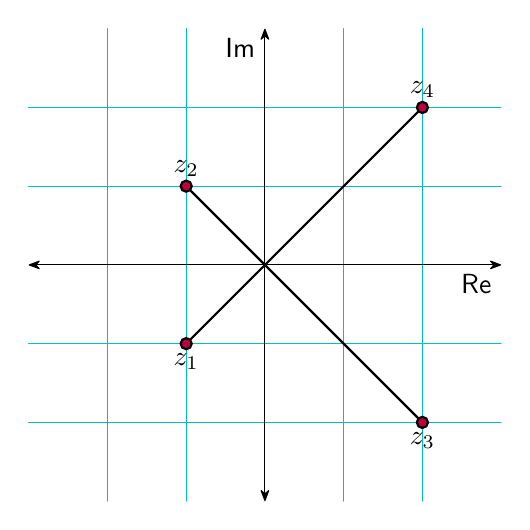
\begin{tikzpicture}

\foreach \i in {-2, -1, 1, 2}
    \draw[line cap = round, Cyan!75!Black] (\i, -3) -- (\i, 3) (-3, \i) -- (3, \i);

\draw[{Stealth[round]}-{Stealth[round]}] (-3,0) -- (3,0);
\draw[{Stealth[round]}-{Stealth[round]}] (0, -3) -- (0, 3);

\node at (3, 0) [anchor=north east] {$\mathsf{Re}$};
\node at (0, 3) [anchor=north east] {$\mathsf{Im}$};

\draw[thick] (-1.0, -1.0) -- (0, 0);
\draw[thick]  (-1.0, 1.0) -- (0, 0);
\draw[thick]  (2.0, -2.0) -- (0, 0);
\draw[thick]  (2.0, 2.0) -- (0, 0);

\node (z1) at (-1, -1) [anchor = north] {$z_1$};
\node (z2) at (-1, 1) [anchor = south] {$z_2$};
\node (z3) at (2, -2) [anchor = north] {$z_3$};
\node (z4) at (2, 2) [anchor = south] {$z_4$};

\draw[thick, fill=purple] (-1.0, -1.0) circle (2pt);
\draw[thick, fill=purple] (-1.0, 1.0) circle (2pt);
\draw[thick, fill=purple] (2.0, -2.0) circle (2pt);
\draw[thick, fill=purple] (2.0, 2.0) circle (2pt);

\end{tikzpicture}

\end{document}

